\section{V11}
\subsection{Subroutinen}
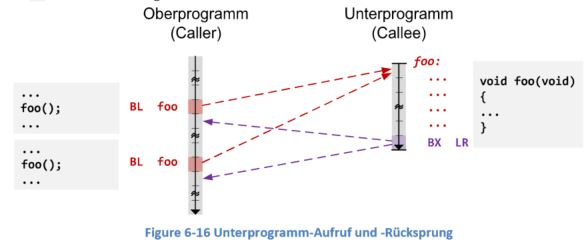
\includegraphics[11cm]{images/subroutinen} 

\subsection{Architecure Producer Call Standart (AAPCS)}
\subsubsection{Regeln}
\begin{itemize}
    \item Bei Funktionsaufrufen werden die Register \textbf{R0-R3} als \textbf{Parameter} an eine C-Funktion verwendet
    \item Werden mehr als vier Funktionsparameter bent"otigt, werden diese vom Caller auf den Stack gelegt und auch wiedervom Caller entfernt.
    \item Die Funktionen müssen die Inhalte der Register \textbf{R4-R11}(falls benutzt) während der Ausführung sichern, um sie am Ende wieder rekonstruieren
    \item Der \textbf{Rückgabewert} einer Subroutine (8-bit, 16-bit,32-bit) wird in den \textbf{Registern R0} übertragen. Handelt es sich um einen 64-bit Rückgabewert, so sind die unteren 32-bit im Register R0 und die oberen 32-bit im Register R1 übertragen
    \item Mit PUSH und POP wird immer eine \textbf{gerade Anzahl von Registern auf dem Stack} gelegt bzw. vom Stack eine \textbf{8-byte Alignment} auf dem Stack einzuhalten
\end{itemize}

\subsubsection{Beispiel}
	Die Parameter"ubergabe bei Funktionen soll mit dem nachfolgenden Beispiel erkl"art werden. \\
	Die Funktion besitzt einen unsigned 8-Bit R"uckgabewert und sechs signed 8-Bit Parameter. \\($\Rightarrow$ 2 Parameter werden "uber den Stack "ubergeben)\\

\begin{minipage}{5cm}
	\begin{enumerate}
		\item \textbf{Stackpointer SP (R13)} wird um 8 nach nach unten verschoben
		\item  Variablen \textit{e} und \textit{f} werden vom Caller auf den Stack gelegt.
		\item \textit{R0 - R3} werden Parameter zugewiesen
		\item Sprung zum Label \textit{foo$\_$4}
		\item \textit{R2, R3, R7, LR} werden auf den Stack gelegt (\textit{SP} wird um 16 nach unten verschoben)
		\item \textit{R7} wird f"ur Zugriff auf \textit{e} und \textit{f} als Framepointer gesetzt.
		\item \textit{R0 - R3} werden auf den Stack gelegt
	\end{enumerate}
\end{minipage}
%
\begin{minipage}{0.25cm}
	\-\
\end{minipage}
%
\begin{minipage}{13cm}
	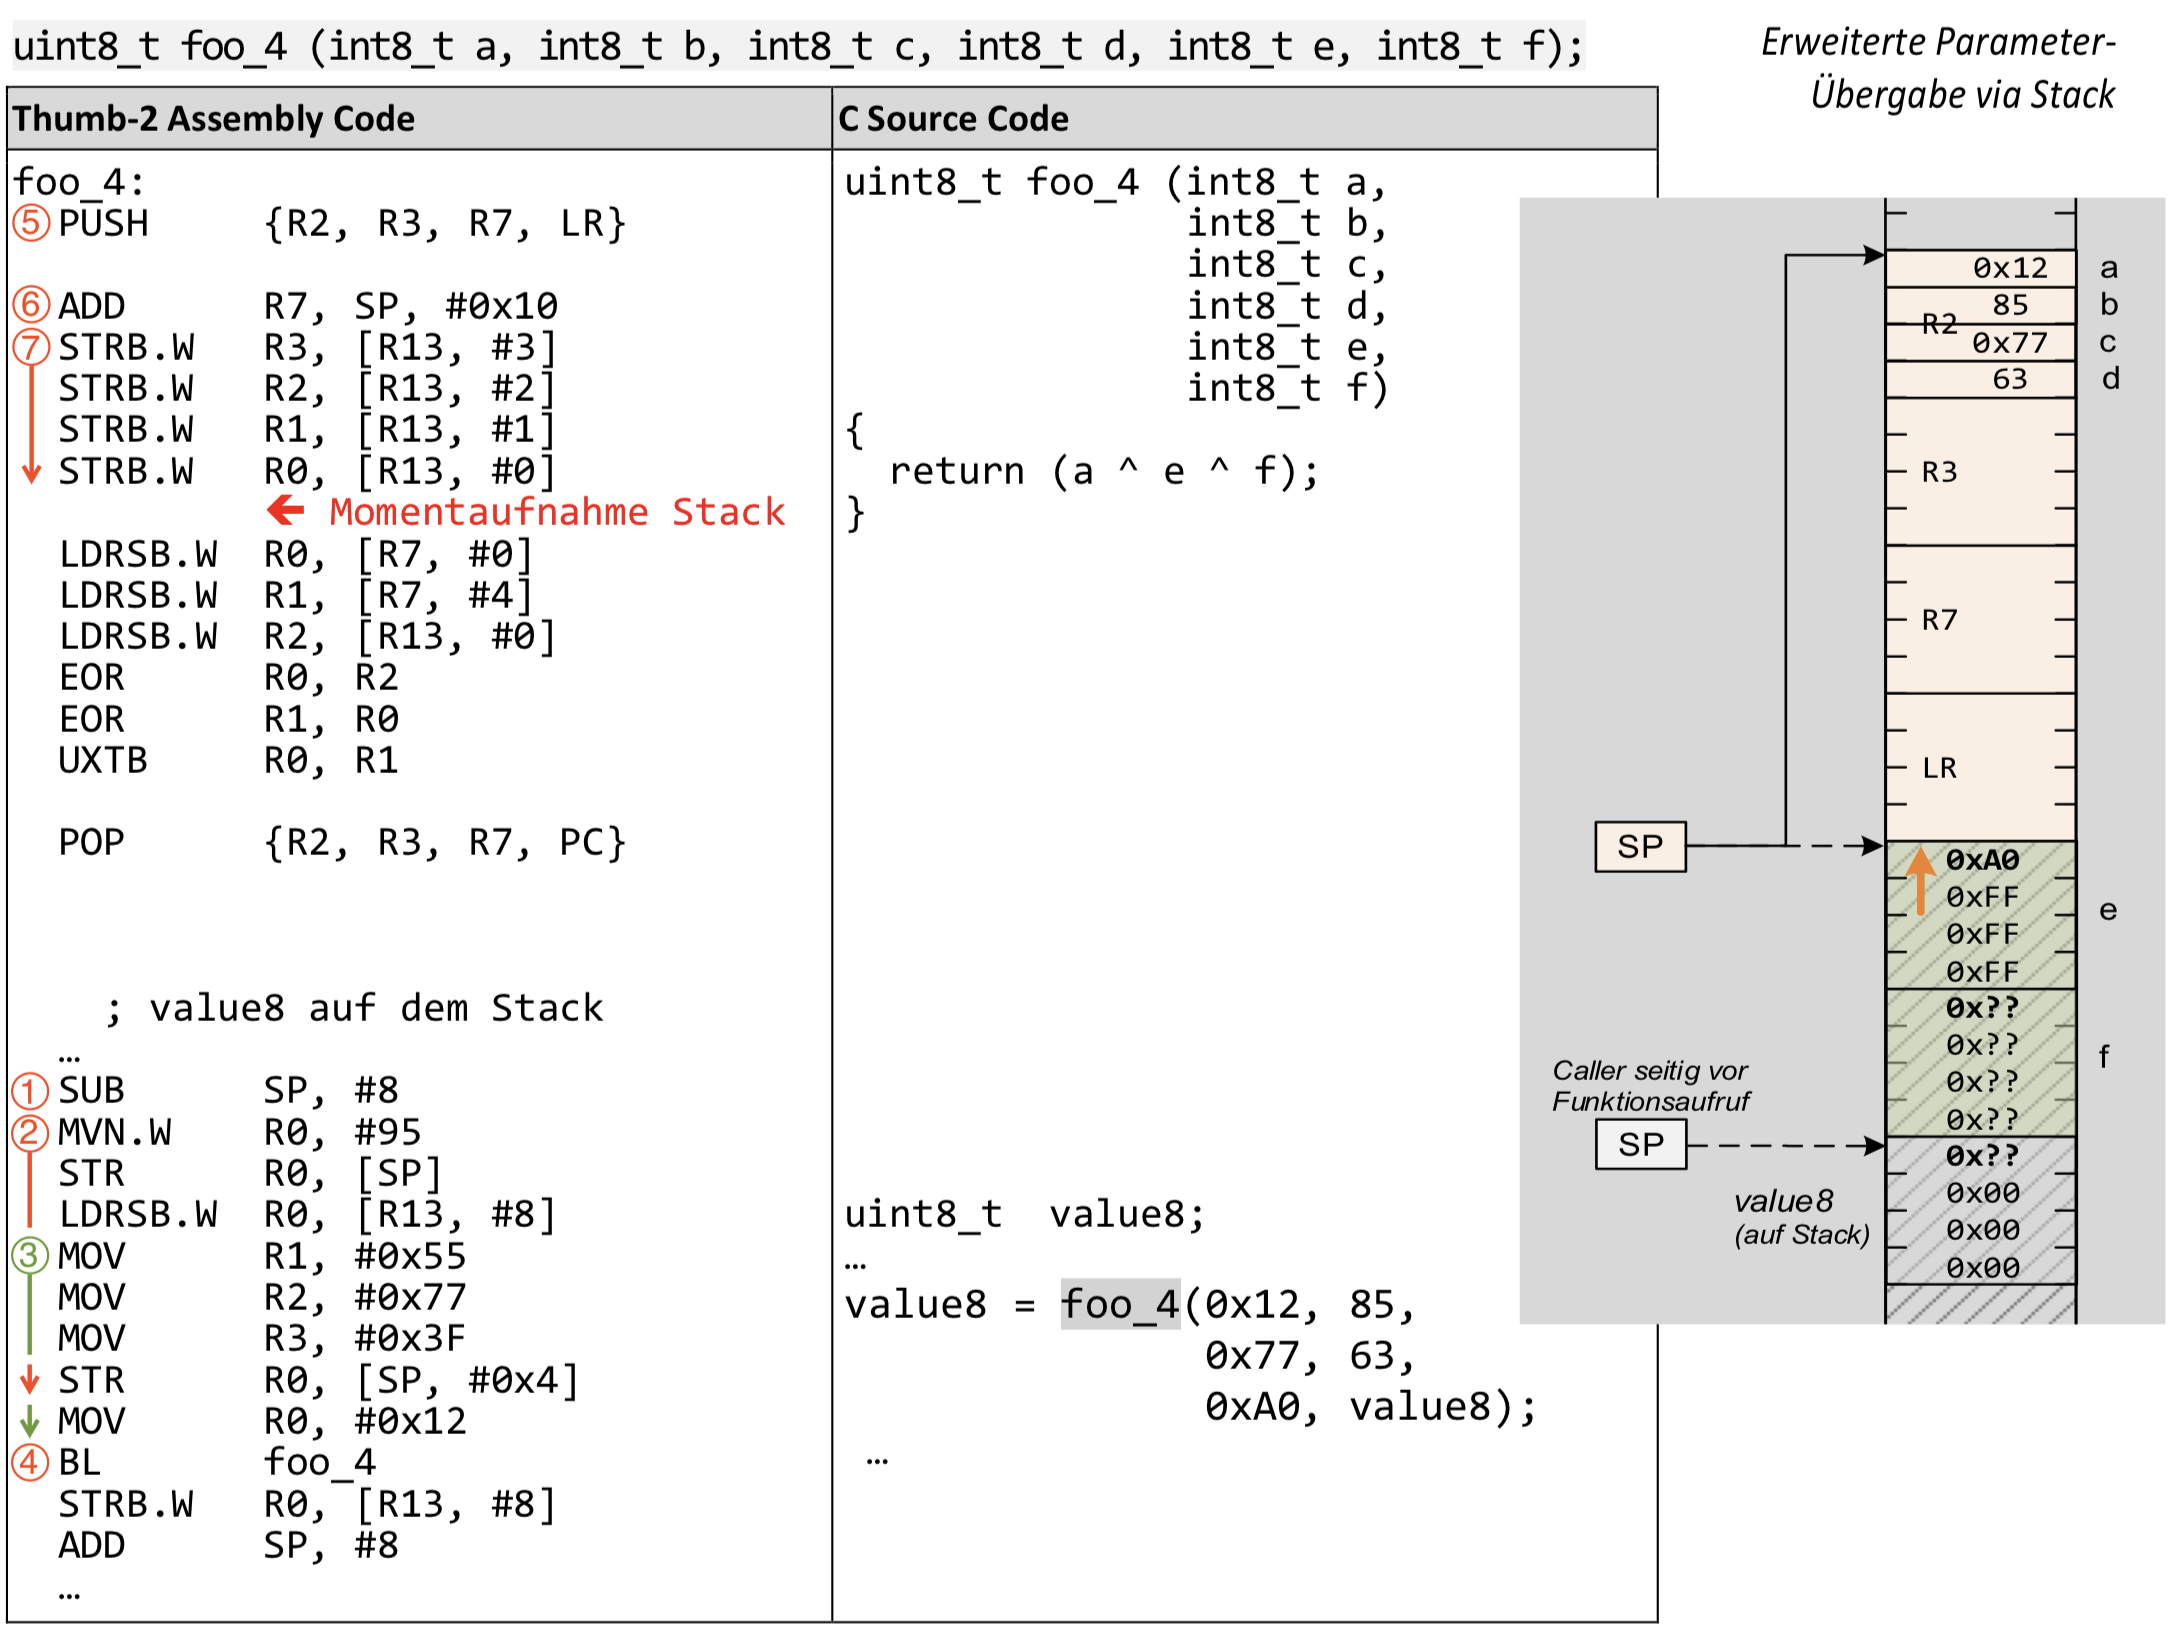
\includegraphics[width=13cm]{images/parameteruebergabe_stack}
\end{minipage}
\newpage